\documentclass[fleqn,12pt]{article}
\usepackage[margin=15mm]{geometry}
\usepackage[T2A]{fontenc}
\usepackage[utf8]{inputenc}
\usepackage[bulgarian]{babel}
\usepackage{indentfirst}
\usepackage{graphicx}
\graphicspath{ {./images/} }

\makeatletter
\newcommand\subsubsubsection{\@startsection{paragraph}{4}{\z@}{-2.5ex\@plus -1ex \@minus -.25ex}{1.25ex \@plus .25ex}{\normalfont\normalsize\bfseries}}
\newcommand\subsubsubsubsection{\@startsection{subparagraph}{5}{\z@}{-2.5ex\@plus -1ex \@minus -.25ex}{1.25ex \@plus .25ex}{\normalfont\normalsize\bfseries}}
\makeatother

\title{Софтуерна архитектура. Проектиране и документиране на софтуерни
архитектури.}
\date{June 2021}

\begin{document}

\maketitle

\section{Дефиниция на софтуерна архитектура. Структури и изгледи  на архитектурата.}
\subsection{Дефиниция на софтуерна архитектура}
Архитектура на дадена софтуерна система е съвкупност от структури, показващи различните софтуерни елементи на системата, външно видимите им свойства и връзките между тях.

Софтуерната архитектура е абстракция, която скрива
детайлите, от които взаимодействието между елементите не зависи. Детайли като алгоритми, представяне на данни, реализация, и т.н. не са
предмет на СА- тя се занимава с поведението и връзките между елементите, разглеждани като ''черни кутии''.

Съгласно дефиницията става ясно, че системите могат да имат (и имат)
повече от една структура. Нито една от тях самостоятелно не
представлява Архитектурата на системата (структура на модулите, на
процесите; елементите може да са обекти, модули, процеси, БД
библиотеки, продукти, екипи и т.н.);
\subsection{Структури и изгледи на архитектурата. }
Структура – съвкупност от софтуерни елементи, техните външно видими свойства и връзките между тях.

Изглед - конкретно документирано представяне на дадена структура. (Двете понятия в голяма степен са взаимозаменяеми).

Структурите се делят на няколко типа.
\subsubsection{Модулни структури}
Елементите в модулните структури са модули – единици работа за изпълнение. Модулите предлагат поглед, ориентиран към реализацията на системата, без значение какво става по време на изпълнението.
Отговарят на въпросите:
\begin {itemize}
\item Коя функционалност в кой модул се реализира? 
\item Кои други модули може да използва (и използва) дадения модул? 
\item Как са свързани модулите по отношение на специализация и генерализация (наследяване)
\end {itemize}
Ще разгледаме няколко типа модулни структури.
\subsubsubsection{ Декомпозиция на модулите}
При тази структура връзките между модулите са от вида “Х е подмодул на У” и модулите биват рекурсивно разбивани на по-прости единици, докато станат лесни за разбиране. Декомпозицията на модулите обуславя в голяма степен възможността за лесна промяна, като обособява логически свързани функционалности на едно място.

\subsubsubsection{Употреба на модулите}
При този вид структура връзките между модулите са от вида “X използва Y”. Структурата за употребата на модули обуславя възможността за лесно добавяне на нова функционалност, обособяване на [в голяма степен] самостоятелни подмножества от функционалност, както и позволява последователната разработка.

\subsubsubsection{Структура на слоевете}
Частен случай на “употреба на модулите”. Модулите са разделени на слоеве, като модулите от слoй N може да ползват услугите само на модули от слой N-1.Слоевете често са реализирани като виртуални машини или обособени подсистеми, които скриват детайлите относно работата си от следващия слой. Подобна структура позволява лесна смяна на даден слой.

\subsubsubsection{Йерархия на класовете}
В терминологията на ООП, модулите се наричат “класове”, а в настоящата структура връзките между класовете са от вида “класът X наследява класа Y” и “обекта X е инстанция на клас Y”. Тази структура обосновава наследяването – защо подобни поведения или въобще функционалности са обособени в супер-класове или пък защо са дефинирани под-класове за обслужване на параметризирани различия.

\subsubsection{Структури на процесите}
Елементите са процеси (или нишки), изпълнявани в системата (компоненти) и комуникационни, синхронизационни или блокиращи операции между тях (конектори); Връзките между тях (attachments) показват как компонентите и конекторите се отнасят помежду си.

\subsubsection{Структури на разположението}
Структурите на разположението показват връзката между софтуерните елементи и елементите на околната среда, в която се намира системата по време на разработката или по време на изпълнението;
Отговарят на въпроситe
\begin {itemize}
\item На кой процесор се изпълнява всеки от елементите? 
\item В кои файлове се записва сорс кода на елементите по време на разработката?
\item Какво е разпределението на софтуерните елементи по екипи, които създават системата?
\end {itemize}

Ще разгледаме няколко типа структури на разпределението.

\subsubsubsection{Структура на внедряването}
Показва как софтуера се разполага върху хардуера и комуникационното оборудване. Елементите са процеси, хардуерни устройства и комуникационни канали. Връзките са напр. “внедрен върху” или “мигрира върху” - показвайки върху кое устройство е разположен даден софтуерен елемент.  Тази структура може да се използва за поглед върху производителността, сигурността и др. на дадена система.

\subsubsubsection{Файлова структура}
Показва кой модул къде се помещава във файловата структура по време на различните фази на реализация. Структурата е критична за управлението на дейностите по разработка и за създаването и поддържането на обкръжение за build-ове.
\subsubsubsection{Разпределение на работата}
Показва кой модул от кой екип се реализира. Елементите са модули и екипи. Екипите често не са списък от хора, а по-скоро виртуална група хора с подходящ опит, знания и умения.



\section{Изисквания към качеството (нефункционални изисквания) на системата}
Качествените изисквания определят как софтуерната система да работи. Качеството е субективно възприятие – различните ЗЛ могат да не одобрят даден дизайн, тъй като тяхната идея за качество се различава от идеята за качество на Архитекта. Бизнес целите определят Качествата, които трябва да бъдат вградени в архитектурата на системата. 

Качествата се разделят на следните три основни групи
\begin{itemize}
\itemТехнологични качества – напр. Надеждност, Изменяемост Производителност, Сигурност, Изпитаемост, Използваемост; 
\itemБизнес качества – напр. време за пускане на продукта на пазара; 
\itemАрхитектурни качества – присъщи на самата архитектура като напр. идейна цялост (влияят косвено върху всички останали качества);
\end{itemize}


Тези Качества поставят изисквания отвъд функционалните (описание на основните възможности на системата и услугите които тя предоставя). Въпреки че функционалността и Качествата са тясно свързани, функционалността често е единственото, което се взема под внимание по време на проектирането. Като следствие много системи се преправят не защото им липсва функционалност, а защото е трудно да се поддържат, трудно е да се смени платформата, не са скалируеми, прекалено са бавни, или пък са несигурни. СА е тази стъпка в процеса на създаването на системата, в която за пръв път се разглеждат качествените изисквания и в зависимост от тях се създават съответните структури, на които се вменява функционалност. За да притежава дадена система изискваните качествени характеристики, те трябва да се имат предвид както по време на проектирането, така и по време на разработката и внедряването.

От перспективата на архитекта, има три основни проблема:
\begin {itemize}
\item Не могат да се тестват - напр. Как бихме тествали дали система е “изменяема”?
\item Често се водят спорове към кое Качество принадлежи даден аспект на системата.
\item За всяко Качество си има собствен речник. Специалистите по Производителност говорят за “събития”, тези по Сигурност – за “атаки”, тези по Надеждност – за откази, и т.н. Всички тези термини всъщност могат да обозначават едно и също събитие.
\end {itemize}

Изискванията за качество трябва да се формализират от архитекта посредством т.н. “сценарии за качество”, за да бъдат те поставени на обективна основа. 

\subsection {Сценарии за качество}
Сценарият за качество е специфично изискване към поведението на системата в дадена ситуация, в светлината на дадено качество.Te играят същата роля за дефиниране на нефункционалните изисквания, каквато роля играят сценариите за употреба (usecases) за дефиниция на функционалните изисквания.  Всеки сценарий описва някаква случка и се характеризира с 
\begin {itemize}
\item Въздействие – състояние/събитие, което подлежи на обработка 
\item Източник – обект (човек, система или нещо друго) който генерира въздействието
\item Обект – системата, или конкретна нейна част, върху която се случва въздействието
\item Контекст – условията, при които се намира обекта по време на обработка на въздействието
\item Резултат – действията, предприети от обекта при случването на въздействието
\item Количествени параметри – резултатът трябва да подлежи на някакви количествени измервания, така че да позволи проверката дали сценарият се изпълнява съгласно изискванията
\end{itemize}
Пример: По време на експлоатация на системата, външен източник изпраща на процеса Х, съобщение за препълване на опашката с потребителски заявки. Х трябва да информира оператора за получаването на съобщението и да продължи работа без прекъсване.

\section{Проектиране на софтуерната архитектура. Процес за проектиране. Избор на
подходящи структури. Последователност на създаване на архитектурата.
Тактики (архитектурни решения) за постигане на желаните качествени
показатели.}

\subsection{Тактики за изправност}
Тактиката е архитектурно решение, чрез което се контролира
резултата на даден сценарий за качество. Наборът от конкретни
тактики се нарича архитектурна
стратегия.
\subsubsection{Откриване и предпазване от откази}
\begin{itemize}
\item Echo
\item Heartbeat, keepalive
\item Изключения – обработват се изключения, които се генерират, когато се стигне до определено състояние на отказ.
\end{itemize}
\subsubsection{Отстраняване на откази}
\begin{itemize}
\item Активен излишък
\item Пасивен излишък
\item Резерва
\item Извеждане от употреба
\item Следене на процесите
\end{itemize}
\subsubsection{Повторно въвеждане в употреба}
\begin{itemize}
\item Паралелна работа
\item Ре-синхронизация на състоянието
\item Контролни точки и rollback
\end{itemize}

\subsection{Тактики за производителност}
\subsubsection{Намаляване на изискванията}
\begin{itemize}
\item Увеличаване на производителността на изчисленията
\item Промяна на периода
\item Промяна на тактовата честота
\item Ограничаване на времето за изпълнение
\item Опашка с краен размер
\end{itemize}
\subsubsection{Управление на ресурсите}
\begin{itemize}
\item Паралелна обработка
\item Излишък на данни/процеси
\item Включване на допълнителни ресурси
\end{itemize}
\subsubsection{Арбитраж на ресурсите}
Когато има недостиг на ресурси (т.е. спор за тях), трябва да има институция, която да решава (т.е. да извършва арбитраж) кое събитие да се обработи с предимство. Това се нарича scheduling. 

\subsection{Тактики за изменяемост}
\subsubsection{Локализиране на промените (намалява броя на директно
засегнатите модули)}
\begin{itemize}
\item Поддръжка на семантична свързаност
\item Очакване на промените
\item Ограничаване на възможните опции
\end{itemize}

\subsubsection{Предотвратяване ефекта на вълната}
\begin{itemize}
\item Скриване на информация
\item Ограничаване на комуникацията
\item Поддръжка на съществуващите интерфейси
\item Използване на посредник
\end{itemize}


\subsubsection{Отлагане на свързването}
\begin{itemize}
\item Включване/изкл./замяна на компоненти
\item Конфигурационни файлове
\item Дефиниране и придържане към протоколи
\end{itemize}


\subsection{Тактики за сигурност}
\subsubsection{Откриване и предпазване от откази}
\begin{itemize}
\item Автентикация на потребителите
\item Оторизация на потребителите
\item Конфиденциалност на данните
\item Интегритет
\item Ограничаване на експозицията
\item Ограничаване на достъпа
\end{itemize}
\subsubsection{Тактики за откриване на атаките}
TODO
\subsubsection{Тактики за възстановяване след атака}
Припокриват се с тактиките за изправност.

\subsection{Тактики за проверяемост}
\begin{itemize}
\item Разделяне на интерфейса от реализацията
\item Вградени модули за мониторинг и журнал
\end{itemize}




\section{Архитектурни стилове}

Архитектурният стил дефинира семейство от системи чрез използването на
шаблон за структурна организация.
Стиловете обуславят речника на компонентите и конекторите, използвани в тях, както и ограниченията в начина на употребата им, напр. Топологията и семантиката на изпълнението им.

\subsection{Pipe-and-filter}

\includegraphics[width=175mm]{paf_simple.png}

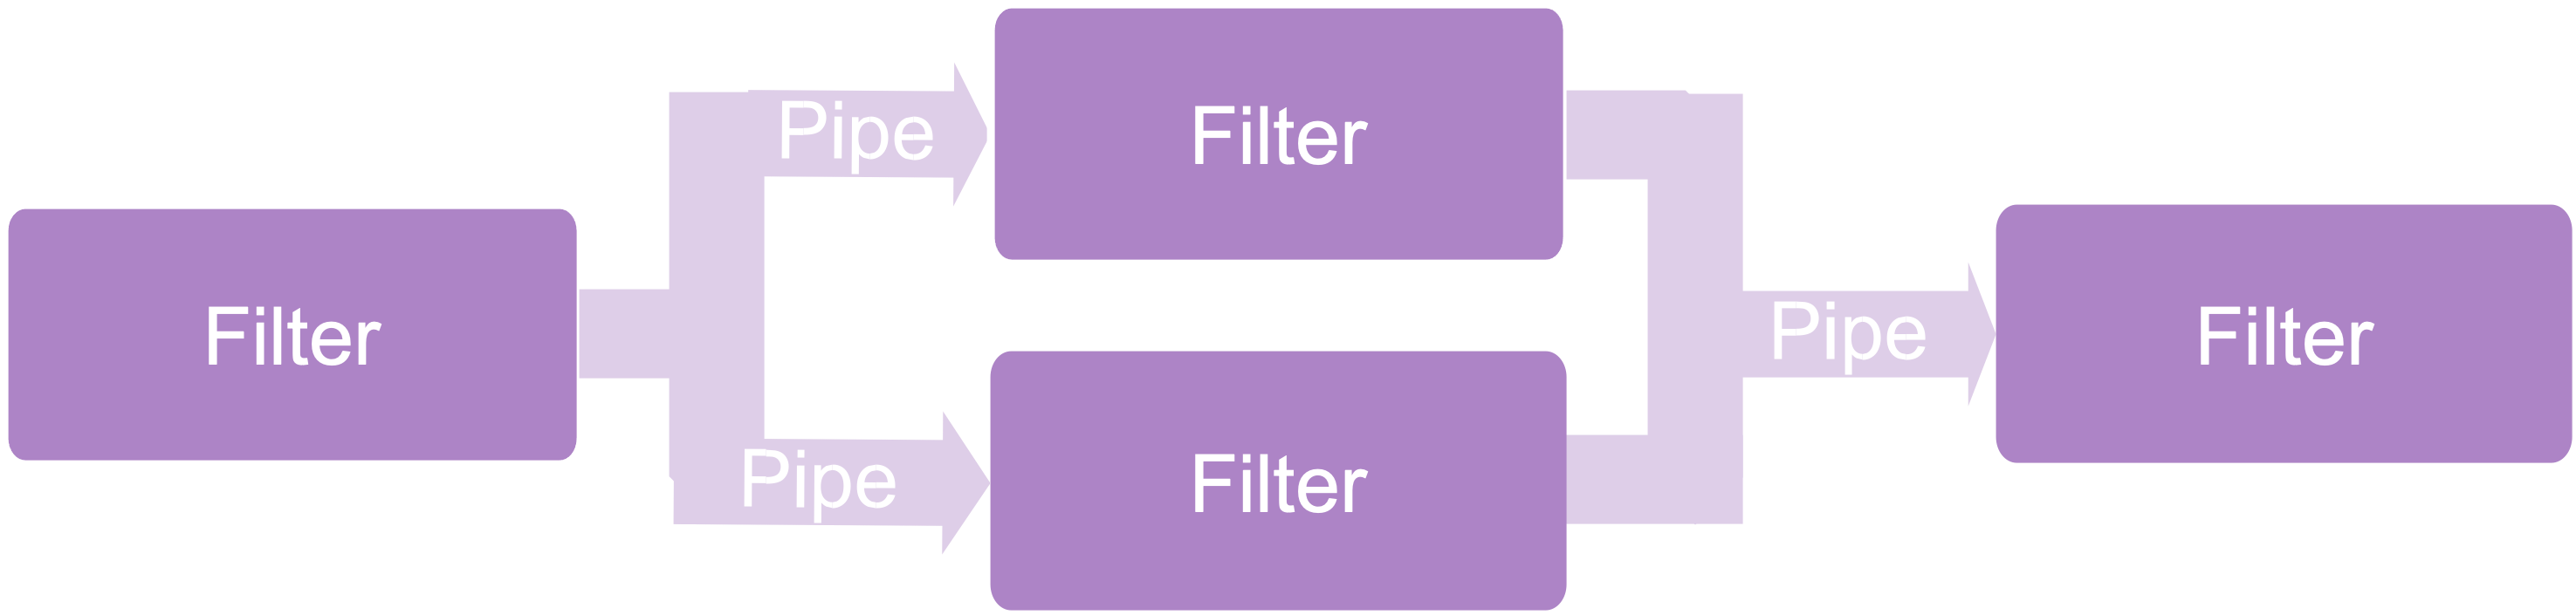
\includegraphics[width=175mm]{paf_branched.png}

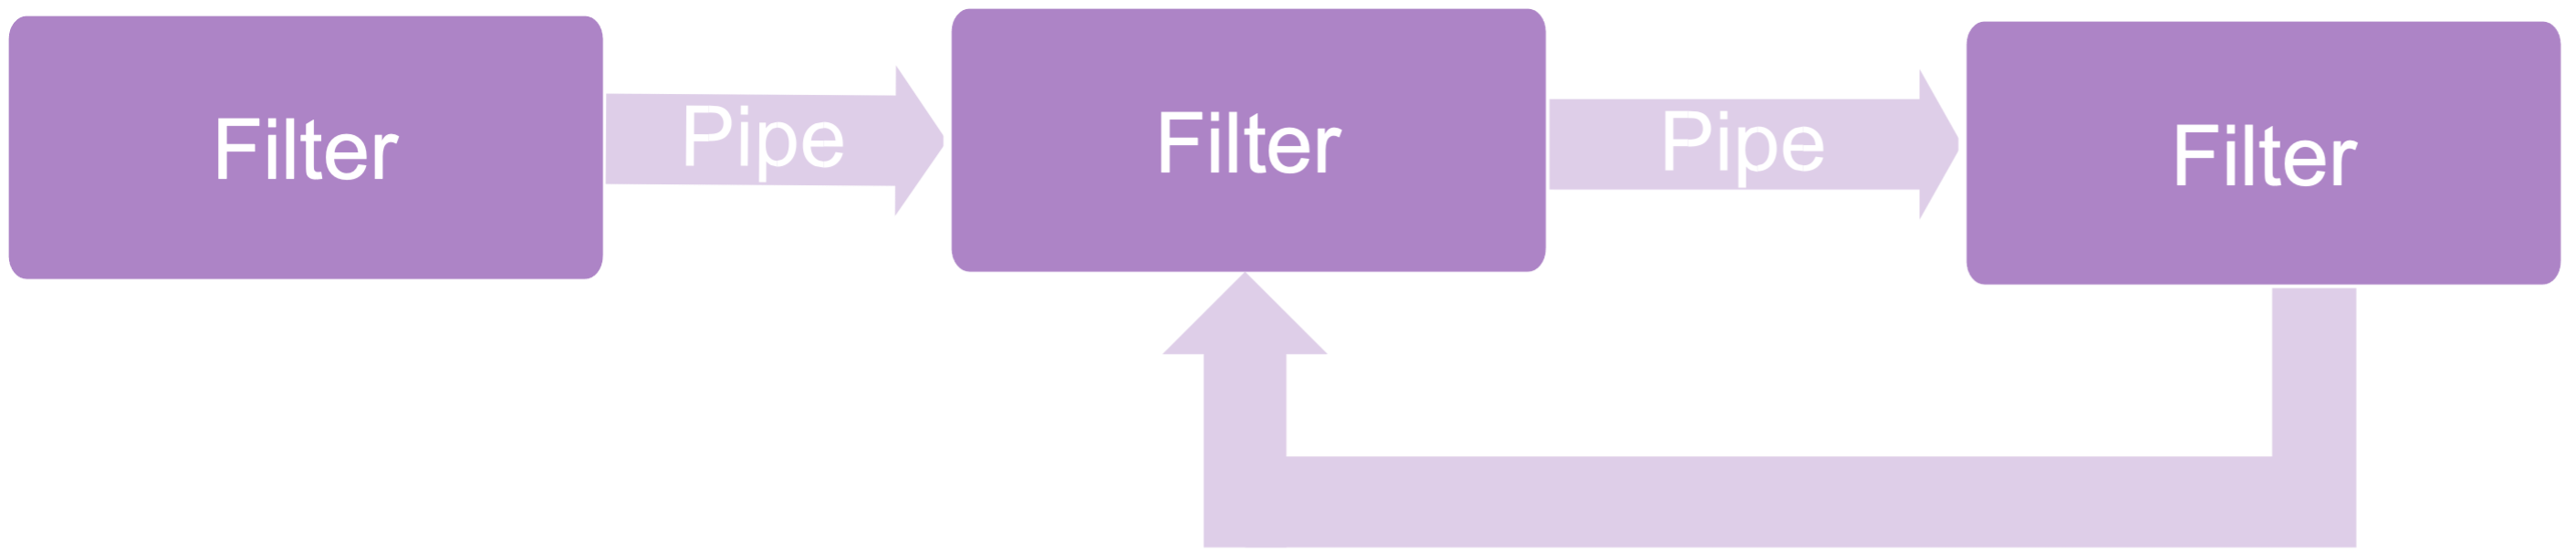
\includegraphics[width=175mm]{paf_loop.png}

Всеки компонент (филтър) на системата има вход и изход. На входа си получава данни, които обработва и извежда на изхода си последователно. Между компонентите има конектори (pipes), които пренасят данните от изхода на даден компонент към входа на следващия. Филтрите нямат никаква информация за съседите си, което прави архитектурата гъвкава и лесна за разбиране. От друга страна, производителността страда заради parse-ването на данни от всеки филтър.

\subsection{Layered}
Тук компонентите са разделени на слоеве, като всеки слой може да предлага услуги на слоя над себе си и да използва услугите на слоя под себе си. Може да разгледаме този стил като частен случай на клиент-сървър архитектурата - всеки слой е клиент за слоя под себе си и сървър за слоя над себе си. Предимствата включват абстракция и лесна изменяемост, докато недостатъците включват компромиси с производителността поради стриктните правила на комуникация, както и по-сложен дизайн процес.

\subsection{Client-server}
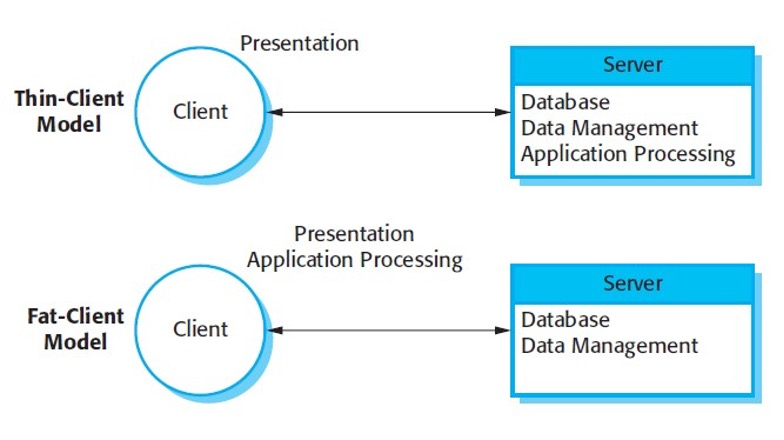
\includegraphics[width=175mm]{client_server.jpg}

Системата е построена като набор от сървъри, предлагащи услуги, и клиенти, които използват тези услуги. Клиентите могат да бъдат “тънки” или “дебели” - дебелите имплементират част от функционалността, а тънките - единствено потребителския интерфейс. Предимствата на този стил са централизираните данни и сигурността, а недостатъците - риск от претоварване, както и нужда от резерви в случай на server failure.

\subsection{Repository/Blackboard}
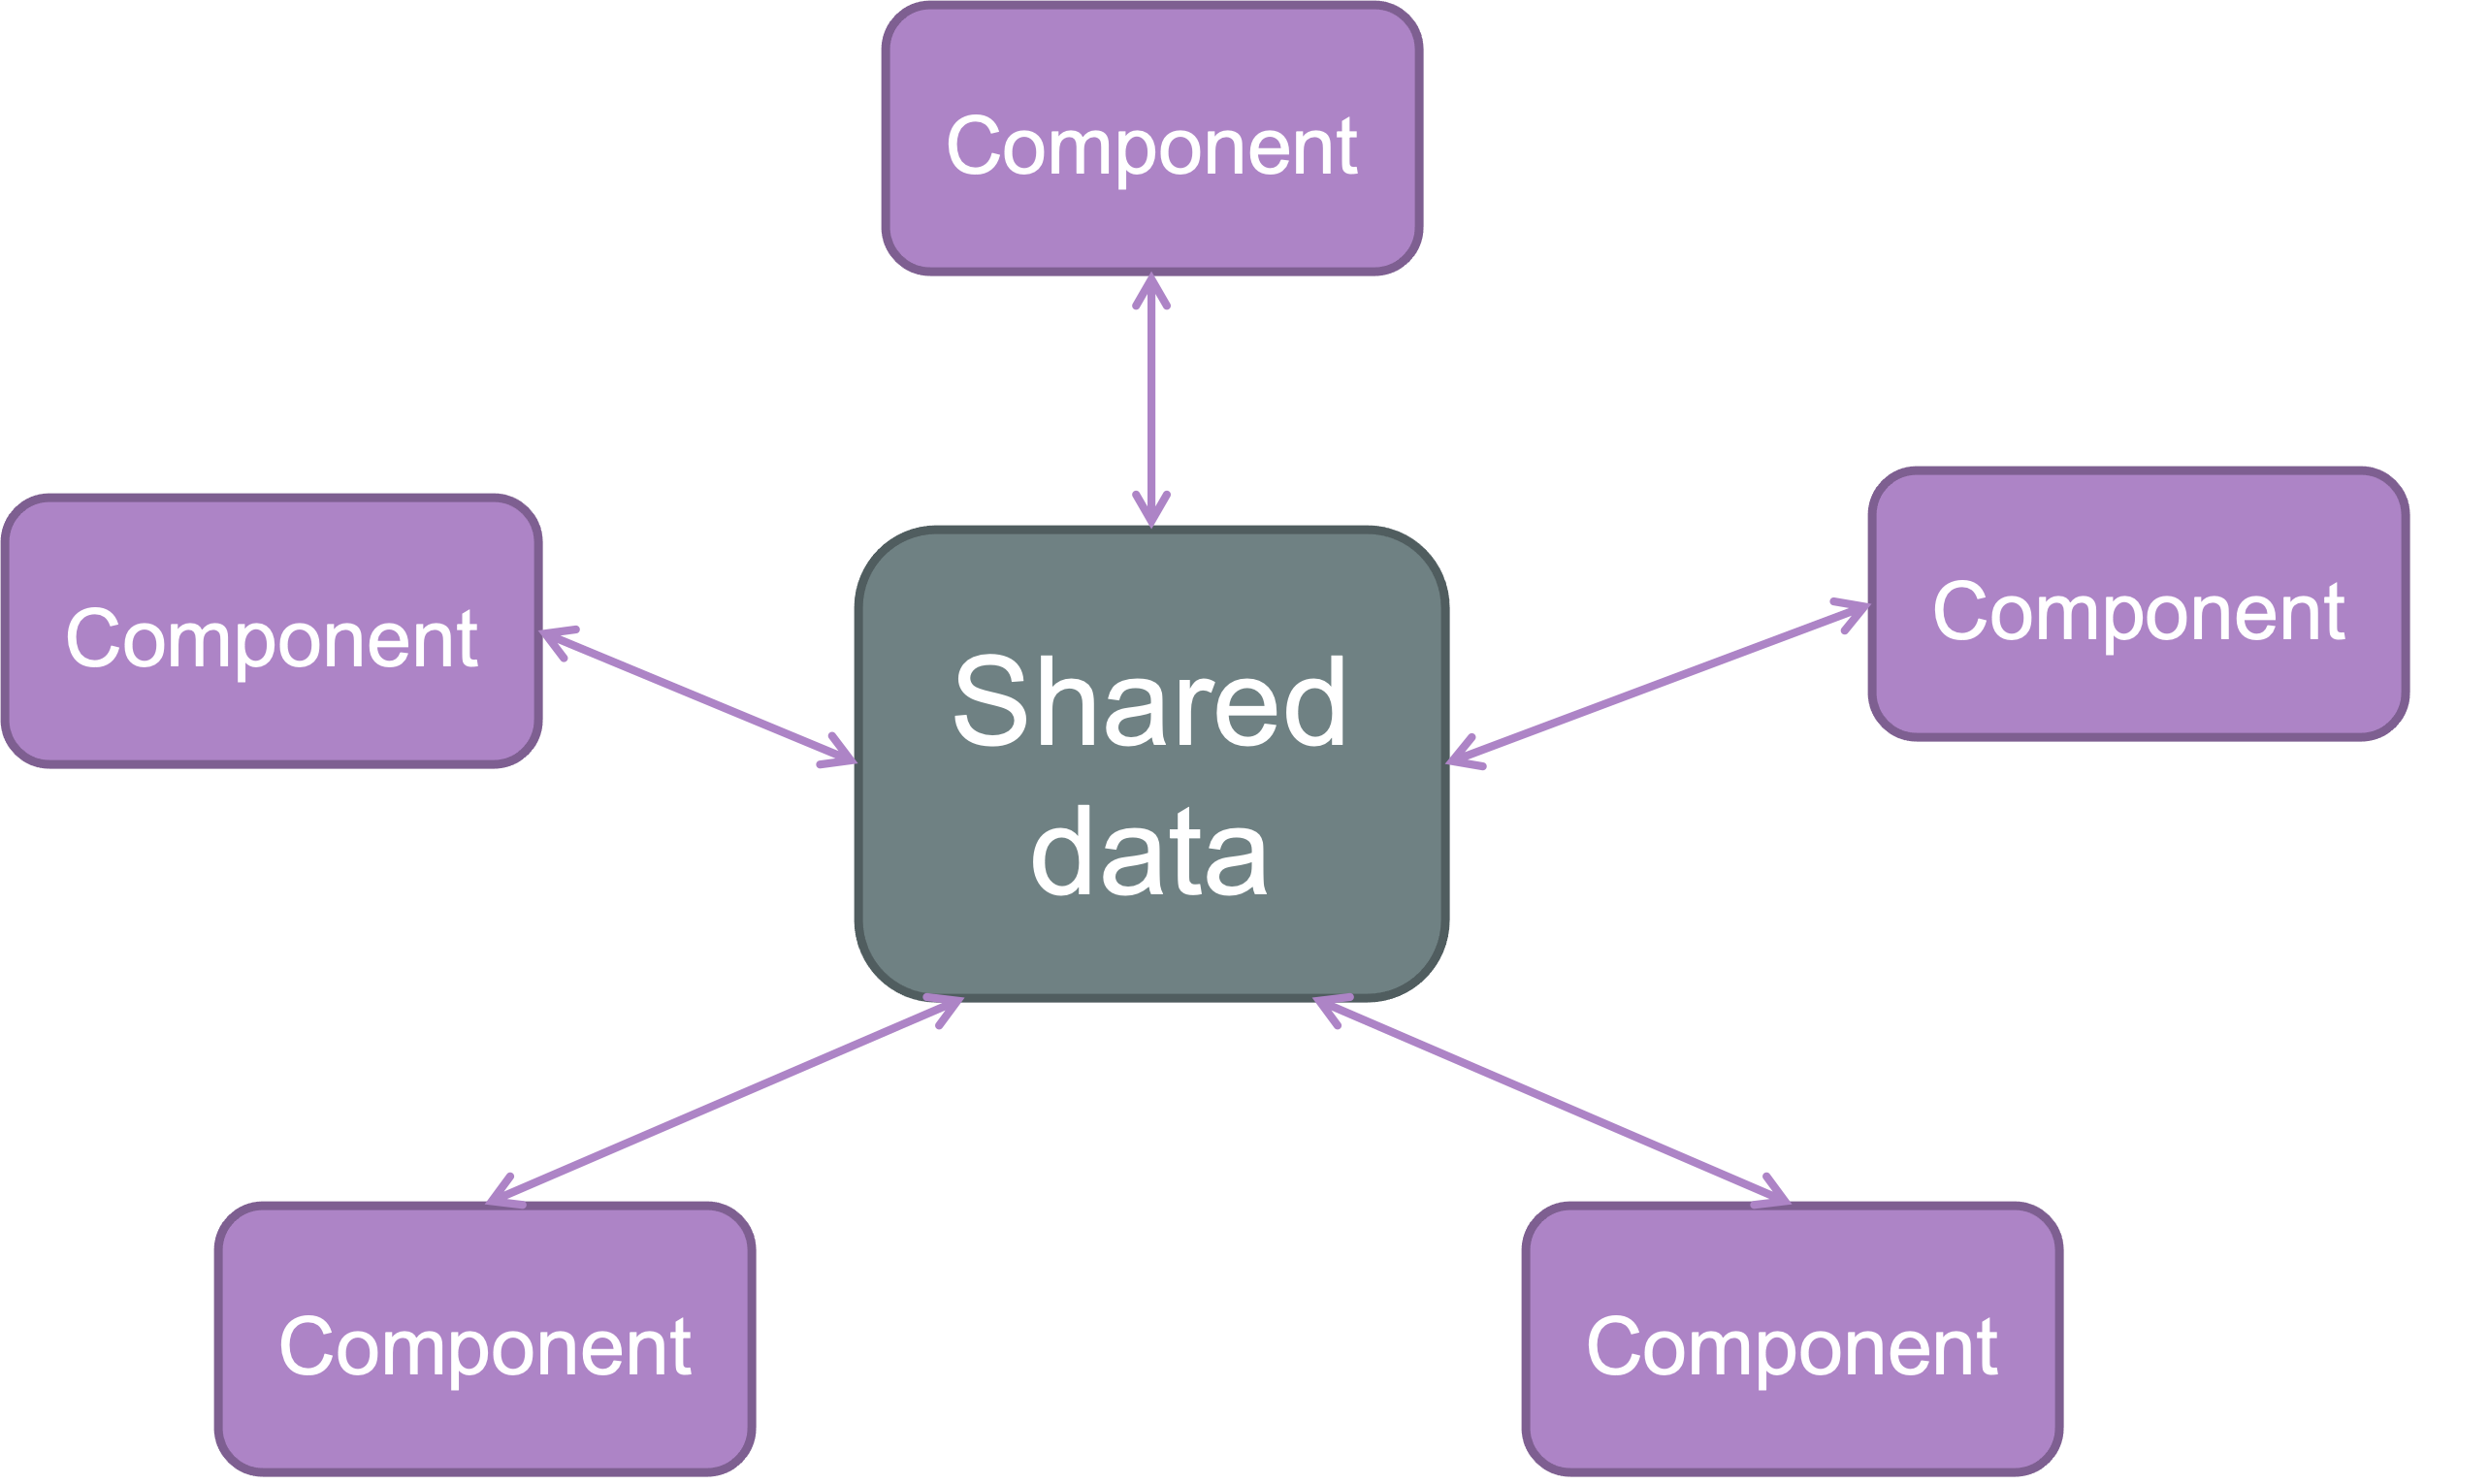
\includegraphics[width=175mm]{shared_memory.png}

Repository и Blackboard са две вариации на архитектурния стил “споделени данни”. Тук самите данни могат да се разглеждат като конектор между компонентите.
При repository вариацията, когато се изпратят данни към общия конектор, всички компоненти биват уведомени. При blackboard вариацията няма подобен механизъм.
Предимствата на този стил включват скалируемост - компоненти се добавят лесно, и висока ефективност при размяна на голямо количество данни. От друга страна, споделената памет представлява bottleneck при голямо количество компоненти и заявки, също така е трудна за имплементация при разпределени системи.

\subsection{Model-View-Controller}
Съдържа три компонента - модел, изглед и контролер.
Моделът представлява знанието - изпраща данни към изгледа, приема заявки за промяна на данните и управлява операциите с тези данни. Изгледа управлява презентацията на данните пред потребителите, а контролера отговаря за взаимодействието с потребителя - натискане на клавиш, кликване и т.н., и изпраща заявки към модела и изгледа за необходимите действия.Този стил прави системата гъвкава и разширяема, но добавя много сложност към архитектурата, както и може да доведе до компромиси с производителността.

\subsection{Implicit invocation/Message passing}
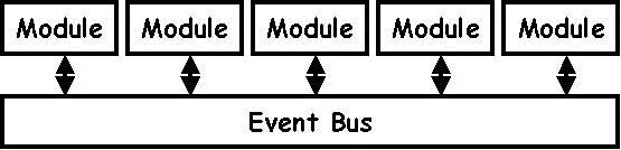
\includegraphics[width=175mm]{implicit_invocation.jpg}

При този стил компонентите си комуникират чрез т.нар. “Събития”. Тези събития може да съдържат както контролни съобщения, така и данни. Компонентите при такава архитектура работят паралелно, а конектора между тях е шина, по която се предават събитията. Предимствата включват сигурност, както и гъвкавост (loose coupling на компонентите). Недостатъците са компромис с надеждността (ако шината умре), както и несигурност (ами ако няма компонент, който да отговори на дадено събити

\section{Документиране на софтуерната архитектура. Предназначение на документацията. Основен принцип на документиране. Съдържание на документацията. Структура на документацията.}

\subsection{Предназначение на документацията.}
Документирането на СА е въпрос на документиране на всички съставляващи я структури поотделно и последващо добавяне на документация, която се отнася за няколко структури.
Документацията е от важност с оглед на това да може в бъдеще системата да бъде
лесно поддържана, безпроблемно изменяна и ясно разказвана на клиенти, потребители.
Трябва да е достатъчно абстрактна, така че да бъде разбрана от нови служители; от друга страна трябва да е достатъчно детайлна, че да послужи за основа на проектирането. 

Документите, предназначени за напр. специалист по сигурността са различни от документите, предназначени за разработчика и различни от документите предназначени за новопостъпили служители.Най-често се създава набор от документи с обогатено съдържание, което указва къде каква информация се съдържа.

\subsection{Основен принцип на документацията}
Документацията се състои от описание на различните структури и когато тя се пише се
мисли най-вече кой ще я чете. Технописецът трябва да се поставя на мястото на
четящия. В документацията различните структури може да се групират по различни
начини в зависимост от това, за кого конкретно е предназначена съответната
документация.


\subsection{Избор на структури, които да бъдат документирани}
Различните перспективи преследват различни цели и имат различно предназначение.
Кои структури ще бъдат документирани зависи от това, кой ще чете документацията
Създава се таблица, комбинират се, слагат се приоритети.

\subsection{Съдържание на документацията}
Няма изграден индустриален стандарт за съдържанието на документацията на дадена структура. Тук разглеждаме 7-елементно съдържание, доказано в практиката

\begin{itemize}
\item Първично представяне -  обикновено графично, често UML. Елементи и връзки между тях, единствено първостепенна информация.
\item Описание на елементите и връзките - детайлно описание на елементите и връзките + второстепенни детайли. Следва да се опише смисъла и ролята на всеки един елемент и връзка, както и поведението и интерфейса (мястото, където два независими софтуерни елемента се срещат и си взаимодействат)  на елементите.
\item Описание на обкръжението - информация за това как елементите от документираната структура си взаимодействат с обкръжението – други системи, интерфейси, протоколи и т.н.
\item Описание на възможните вариации - често архитектурата е изградена така, че да позволява варианти за някои от детайлите, като конкретния вариант може да бъде избран на по-късен етап. Обикновено се дават като ограничителни условия и изисквания. Трябва да бъдат описани вариантите и условията.
\item Архитектурна обосновка - обяснява на заинтересованите лица защо структурата е проектирана по начина по който е описана. Обоснование на взетите решения, алтернативи, резултати, предположения.
\item Терминологичен речник - кратко описание на използваната стандартна и нововъведена терминология
\item Допълнителна информация - всичко останало, административна информация. Съдържа описание на съдържанието си.
\end{itemize}

\subsection{Структура на документацията}
TODO




\end{document}
